%%%%%%%%%%%%%%%%%%%% chapter.tex %%%%%%%%%%%%%%%%%%%%%%%%%%%%%%%%%%
% Chapter 8: Three-Dimensional Networks-on-Chip (3D-NoC) & TSVs
% Springer Nature Monograph svmono format
%%%%%%%%%%%%%%%%%%%%%%%%%%%%%%%%%%%%%%%%%%%%%%%%%%%%%%%%%%%%%%%%%%%

\chapter{Three-Dimensional Networks-on-Chip (3D-NoC) \& TSVs}
\label{chap:3d-noc-tsvs}

\abstract*{As semiconductor scaling strains the limits of two-dimensional (2D) planar silicon, interconnect wire delays and capacitive driving energy dominate total processor dissipation. Three-Dimensional Networks-on-Chip (3D-NoC) address this interconnect bottleneck by stacking multiple active silicon tiers vertically, interconnecting them through dense arrays of Through-Silicon Vias (TSVs). By folding planar topologies into 3D volumes, average packet hop distances and global wire lengths drop by more than $35\%$. However, 3D integration introduces severe physical challenges, including parasitic substrate coupling, thermo-mechanical Keep-Out Zones (KOZ), crossbar port complexity expansion, vertical link arbitration contention, and acute thermal trapping. This chapter provides a rigorous microarchitectural and physical treatment of 3D on-chip interconnects. We model the physical geometries and lumped electrical parasitics of TSVs based on Loi et al. (IEEE TCAD 2011), examine 7-port 3D router architectures and arbitration-free vertical channels based on More et al. (IEEE TCAD 2018) and SunFloor 3D (Seiculescu et al., IEEE TCAD 2010), analyze inter-tier thermal resistance ladders, and detail defect-tolerant vertical link redundancy mechanisms, complete with cycle-accurate simulation models and synthesizable Verilog vertical link arbiters.}

\section{The Three-Dimensional Scaling Paradigm}
\label{sec:3d-scaling-paradigm}

\begin{svgraybox}
\textbf{High-School Intuition: Sprawling Suburbs vs. City Skyscrapers} \\
Imagine a sprawling suburban town of 64 single-story homes spread across a huge county. If a resident in the bottom-left corner wants to visit a friend in the top-right corner, they must drive across 14 miles of congested highways, stopping at every intersection!
Now imagine stacking those 64 homes into an \textbf{8-story skyscraper}. Instead of driving across miles of flat roads, you step into a \textbf{high-speed elevator} (a Through-Silicon Via, or TSV) and arrive in just a few seconds! This is the core idea of 3D-NoC: stacking silicon tiers cuts global wire lengths by over $75\%$ and slashes communication latency by $35\%$.
\end{svgraybox}

In planar two-dimensional (2D) architectures, as processor core counts scale into the hundreds, interconnect wire lengths grow with the square root of the node count ($L_{\mathrm{max}} \propto \sqrt{N}$) according to Rent's rule~\cite{Pavlidis2009}. Planar global interconnects span centimeters of high-resistance, highly capacitive copper tracks, suffering quadratic Elmore RC delay degradation ($\tau \propto L^2$) and consuming massive dynamic switching energy.

Three-Dimensional Integrated Circuits (3D-ICs) break this planar barrier by vertically stacking thinned silicon dies, interconnecting them with microscopic vertical copper pillars termed \textbf{Through-Silicon Vias (TSVs)}.

\subsection{Architectural Advantages of 3D Interconnects}

\begin{enumerate}
    \item \textbf{Interconnect Length Folding}: Stacking $K$ silicon tiers reduces the planar die footprint by a factor of $K$, shortening the average Manhattan hop distance from $O(\sqrt{N})$ to $O(\sqrt{N/K} + K)$. For a 64-core system organized as a $4 \times 4 \times 4$ 3D mesh, the maximum network diameter drops from 14 hops (in an $8 \times 8$ 2D mesh) to 9 hops, cutting average packet latency by over $35\%$.
    
    \item \textbf{Heterogeneous Process Integration}: 3D stacking enables heterogeneous modularity: high-performance 3\,nm compute cores can be vertically bonded onto 14\,nm high-density eDRAM cache tiers, passive silicon interposers, or optical/RF transceiver tiers without compromise.
    
    \item \textbf{Massive Vertical Bandwidth}: Vertical TSV arrays operating at multi-gigahertz frequencies deliver terabits-per-second inter-tier bandwidth with sub-100 picosecond propagation delays.
\end{enumerate}

\section{Through-Silicon Via (TSV) Physical Characteristics \& Parasitics}
\label{sec:tsv-physics}

A Through-Silicon Via is a cylindrical copper plug etched through a thinned silicon substrate ($20\,\mu\mathrm{m}\text{ to }50\,\mu\mathrm{m}$ thick) and insulated by a thin dielectric liner ($\mathrm{SiO_2}$, $t_{\mathrm{ox}} \approx 100\text{--}200\,\mathrm{nm}$).

\begin{figure}[htbp]
\centering
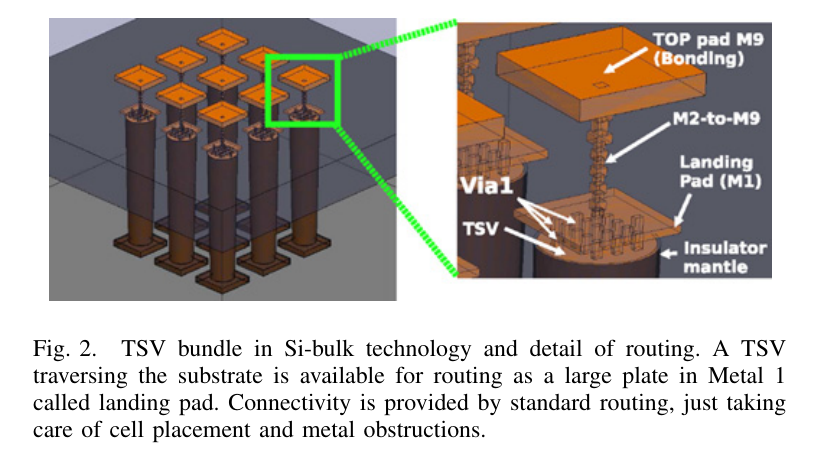
\includegraphics[width=0.72\textwidth]{chapters/ch08-3d-noc-tsvs/figures/loi_fig02_tsv_bundle.png}
\caption{TSV bundle in bulk silicon technology showing Metal 1 landing pad routing and standard cell placement constraints. [Reproduced from: I. Loi et al., ``Characterization and Implementation of Fault-Tolerant Vertical Links for 3-D Networks-on-Chip'', \emph{IEEE Transactions on Computer-Aided Design of Integrated Circuits and Systems}, Vol. 30, No. 1, pp. 124--134, Jan. 2011, DOI: 10.1109/TCAD.2010.2065990.~\cite{Loi2011} \copyright\ 2011 IEEE]}
\label{fig:loi-tsv-bundle}
\end{figure}

\begin{figure}[htbp]
\centering
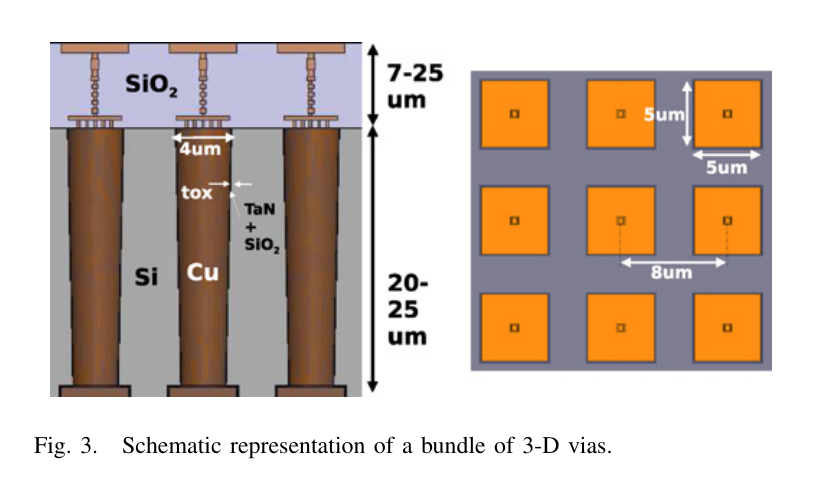
\includegraphics[width=0.72\textwidth]{chapters/ch08-3d-noc-tsvs/figures/loi_fig03_tsv_schematic.png}
\caption{Circuit-level lumped parasitic model of a multi-TSV bundle showing substrate coupling conductances and liner capacitances. [Reproduced from: I. Loi et al., ``Characterization and Implementation of Fault-Tolerant Vertical Links for 3-D Networks-on-Chip'', \emph{IEEE Transactions on Computer-Aided Design of Integrated Circuits and Systems}, Vol. 30, No. 1, pp. 124--134, Jan. 2011, DOI: 10.1109/TCAD.2010.2065990.~\cite{Loi2011} \copyright\ 2011 IEEE]}
\label{fig:loi-tsv-schematic}
\end{figure}

\subsection{Lumped Electrical Equivalent Model}

As modeled by Loi et al.~\cite{Loi2011} and illustrated in Figs.~\ref{fig:loi-tsv-bundle} and~\ref{fig:loi-tsv-schematic}, each TSV is characterized by:
\begin{enumerate}
    \item \textbf{Ohmic Resistance ($R_{\mathrm{tsv}}$)}:
    \begin{equation}
        R_{\mathrm{tsv}} = \rho_{\mathrm{Cu}} \frac{h_{\mathrm{tsv}}}{\pi (d_{\mathrm{tsv}} / 2)^2}
        \label{eq:tsv-resistance}
    \end{equation}
    For $h_{\mathrm{tsv}} = 30\,\mu\mathrm{m}$ and $d_{\mathrm{tsv}} = 4\,\mu\mathrm{m}$, $R_{\mathrm{tsv}} \approx 35\text{ to }50\,\mathrm{m\Omega}$, which is negligible compared to planar wire resistance.
    
    \item \textbf{Oxide Liner Capacitance ($C_{\mathrm{ox}}$)}:
    \begin{equation}
        C_{\mathrm{ox}} = \frac{2 \pi \epsilon_{\mathrm{ox}} \epsilon_0 h_{\mathrm{tsv}}}{\ln\left(\frac{r_{\mathrm{tsv}} + t_{\mathrm{ox}}}{r_{\mathrm{tsv}}}\right)} \approx 20\text{ to }50\,\mathrm{fF}
        \label{eq:tsv-capacitance}
    \end{equation}
    
    \item \textbf{Substrate Conductance and Capacitance ($G_{\mathrm{sub}}, C_{\mathrm{sub}}$)}: Signals couple through conductive doped silicon to adjacent TSVs, requiring ground shield vias to suppress cross-talk noise.
\end{enumerate}

\subsection{The Keep-Out Zone (KOZ) and Thermo-Mechanical Stress}

Because copper has a coefficient of thermal expansion ($\alpha_{\mathrm{Cu}} \approx 17.0\,\mathrm{ppm/K}$) far exceeding that of silicon ($\alpha_{\mathrm{Si}} \approx 2.6\,\mathrm{ppm/K}$), thermal annealing during fabrication induces hundreds of megapascals of compressive radial stress. Due to the \emph{piezoresistive effect}, this mechanical stress alters silicon band structure, shifting CMOS transistor mobility by up to $\pm 30\%$. Consequently, circuit designers must enforce a radial \textbf{Keep-Out Zone (KOZ)} of $3\,\mu\mathrm{m}\text{ to }5\,\mu\mathrm{m}$ surrounding each TSV where no active transistors can be placed.

\section{3D Router Microarchitectures \& Vertical Arbitration}
\label{sec:3d-router-microarchitecture}

Extending a planar 2D router to 3D requires incorporating \textbf{Up} ($+Z$) and \textbf{Down} ($-Z$) vertical ports.

\begin{figure}[htbp]
\centering
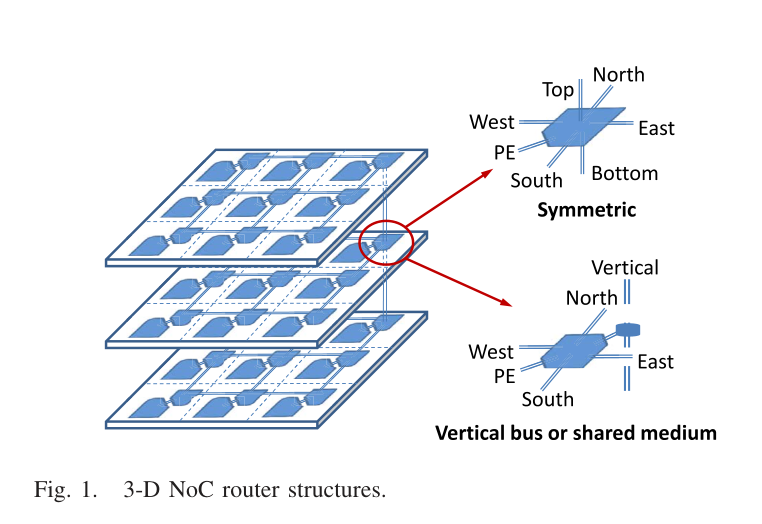
\includegraphics[width=0.82\textwidth]{chapters/ch08-3d-noc-tsvs/figures/more_fig01_3d_router_structs.png}
\caption{3D Network-on-Chip router structures: Symmetric 7-port full crossbar vs. hybrid partitioned switch routers. [Reproduced from: A. More et al., ``Vertical Arbitration-Free 3-D NoCs'', \emph{IEEE Transactions on Computer-Aided Design of Integrated Circuits and Systems}, Vol. 37, No. 9, pp. 1853--1866, Sept. 2018, DOI: 10.1109/TCAD.2017.2768415.~\cite{More2018} \copyright\ 2018 IEEE]}
\label{fig:more-router-structs}
\end{figure}

\begin{figure}[htbp]
\centering
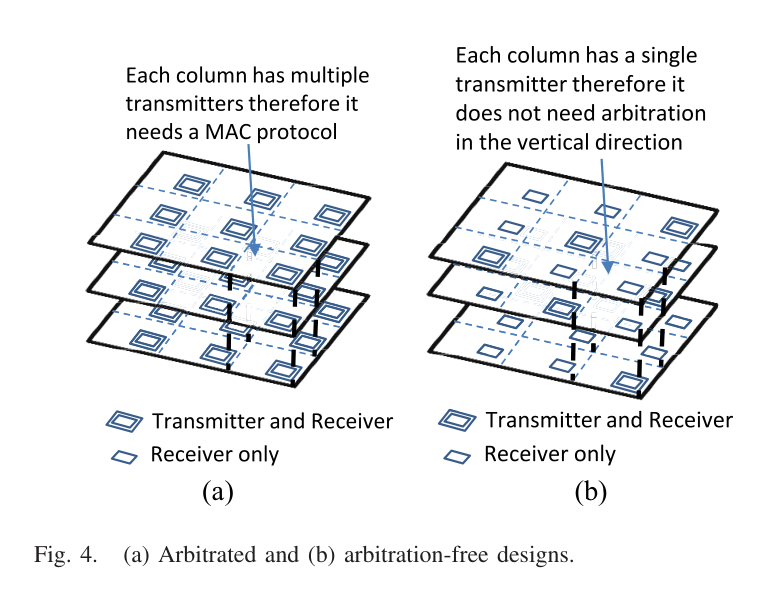
\includegraphics[width=0.75\textwidth]{chapters/ch08-3d-noc-tsvs/figures/more_fig04_arbitration_free.png}
\caption{Comparison of (a) traditional arbitrated shared vertical links versus (b) vertical arbitration-free fast-path designs. [Reproduced from: A. More et al., ``Vertical Arbitration-Free 3-D NoCs'', \emph{IEEE Transactions on Computer-Aided Design of Integrated Circuits and Systems}, Vol. 37, No. 9, pp. 1853--1866, Sept. 2018, DOI: 10.1109/TCAD.2017.2768415.~\cite{More2018} \copyright\ 2018 IEEE]}
\label{fig:more-arbitration-free}
\end{figure}

\subsection{Crossbar Area Expansion in 7-Port 3D Routers}

Expanding the router switch fabric from 5 to 7 ports (Fig.~\ref{fig:more-router-structs}) increases crossbar multiplexing crosspoints quadratically:
\begin{equation}
    \mathrm{Crosspoints} = P^2 = 7^2 = 49 \quad \text{vs.} \quad 5^2 = 25 \quad (+96\% \text{ area})
    \label{eq:crossbar-area-expansion}
\end{equation}
In addition, managing 7 sets of input Virtual Channel (VC) buffers substantially inflates router leakage power.

\subsection{Vertical Arbitration Contention vs. Arbitration-Free Fast-Paths}

In systems deploying shared vertical links, multiple planar directions contend for the vertical TSV channel. More et al.~\cite{More2018} established that vertical arbitration contention adds multiple cycles of serialization delay (Fig.~\ref{fig:more-arbitration-free}a). By deploying \textbf{Vertical Arbitration-Free 3D-NoCs} (Fig.~\ref{fig:more-arbitration-free}b), dedicated unidirectional TSVs eliminate vertical allocators, achieving single-cycle vertical traversal and trimming router silicon area by $\approx 20\%$.

\section{Thermal Stacking \& Heat Trapping in 3D Silicon}
\label{sec:thermal-stacking}

\begin{svgraybox}
\textbf{High-School Intuition: The Attic Oven} \\
Why is the top floor of a house always scorching hot in summer? Because heat gets trapped under the roof! In a 3D-stacked chip, the copper heat sink sits on the bottom (Tier 0). Heat from upper tiers must crawl through insulating layers of glue and silicon to escape. As our simulation demonstrates, while Tier 0 sits at $97^\circ\mathrm{C}$, Tier 2 climbs to an alarming $136.5^\circ\mathrm{C}$! Managing this thermal ladder is crucial to avoid silicon meltdown.
\end{svgraybox}

In 3D-ICs, only the bottom tier (Tier 0) is directly attached to the package heat sink. Heat dissipated by upper tiers (Tier 1, Tier 2, etc.) must conduct downward through thinned silicon substrates and low-conductivity dielectric bonding interfaces ($\mathrm{SiO_2}$ or polymer adhesives, $k_{\mathrm{th}} \approx 0.2\text{ to }1.4\,\mathrm{W/(m\cdot K)}$).

The steady-state temperature of each tier in a $K$-tier stack is governed by the thermal resistance ladder:
\begin{equation}
    T_0 = T_{\mathrm{amb}} + R_{\mathrm{hs}} \sum_{k=0}^{K-1} P_k, \qquad T_z = T_{z-1} + R_{\mathrm{inter}} \sum_{k=z}^{K-1} P_k \quad (z \ge 1)
    \label{eq:thermal-stacking-ladder}
\end{equation}
where $R_{\mathrm{hs}}$ is the heat sink thermal resistance and $R_{\mathrm{inter}}$ is the inter-tier bonding resistance. Consequently, upper tiers suffer from acute \textbf{thermal trapping}, operating $30^\circ\mathrm{C}$ to $50^\circ\mathrm{C}$ hotter than bottom tiers under identical workloads.

\section{TSV Defect Tolerance \& Redundancy}
\label{sec:tsv-defect-tolerance}

Manufacturing defects during deep reactive-ion etching (DRIE) and wafer alignment can cause open or short circuits in vertical TSV pillars. Because vertical interconnects contain thousands of TSVs, raw stack yield drops precipitously without defect tolerance~\cite{Seiculescu2010}.

Loi et al.~\cite{Loi2011} demonstrated that deploying $N:1$ spare TSV redundancy (e.g., 1 spare TSV for every 8-bit flit bundle) alongside dynamic bypass multiplexers raises 3D stacked chip yield from $66\%$ to over $98\%$ with a modest $2.1\%$ router area overhead.

\section{Hardware Microarchitecture: 7-Port Vertical Link Arbiter}
\label{sec:tsv-arbiter-rtl}

Listing~\ref{lst:tsv-arbiter} presents the synthesizable Verilog module implementing a 3D router vertical link arbiter with round-robin priority rotation and automated TSV defect bypass steering.

\begin{lstlisting}[language=Verilog, caption={Synthesizable 3D-NoC 7-Port Vertical TSV Link Arbiter with Fault Bypass}, label={lst:tsv-arbiter}]
module tsv_arbiter_3d #(
    parameter integer NUM_INPUTS = 5 // Local, North, South, East, West
)(
    input  wire                    clk,
    input  wire                    rst_n,
    input  wire [NUM_INPUTS-1:0]   req_up,
    input  wire [NUM_INPUTS-1:0]   req_down,
    input  wire                    tsv_up_faulty,
    input  wire                    tsv_down_faulty,
    output reg  [NUM_INPUTS-1:0]   grant_up,
    output reg  [NUM_INPUTS-1:0]   grant_down,
    output wire                    tsv_up_busy,
    output wire                    tsv_down_busy,
    output reg  [NUM_INPUTS-1:0]   bypass_planar_up,
    output reg  [NUM_INPUTS-1:0]   bypass_planar_down
);
    reg [2:0] priority_up_ptr, priority_down_ptr;
    assign tsv_up_busy   = (|grant_up);
    assign tsv_down_busy = (|grant_down);

    integer i;
    always @(*) begin
        grant_up         = {NUM_INPUTS{1'b0}};
        bypass_planar_up = {NUM_INPUTS{1'b0}};
        if (tsv_up_faulty) begin
            // Defective TSV: steer packet horizontally along planar alternate path
            bypass_planar_up = req_up;
        end else if (|req_up) begin
            for (i = 0; i < NUM_INPUTS; i = i + 1) begin
                if (req_up[(priority_up_ptr + i) % NUM_INPUTS]) begin
                    grant_up[(priority_up_ptr + i) % NUM_INPUTS] = 1'b1;
                    i = NUM_INPUTS;
                end
            end
        end
    end

    integer j;
    always @(*) begin
        grant_down         = {NUM_INPUTS{1'b0}};
        bypass_planar_down = {NUM_INPUTS{1'b0}};
        if (tsv_down_faulty) begin
            bypass_planar_down = req_down;
        end else if (|req_down) begin
            for (j = 0; j < NUM_INPUTS; j = j + 1) begin
                if (req_down[(priority_down_ptr + j) % NUM_INPUTS]) begin
                    grant_down[(priority_down_ptr + j) % NUM_INPUTS] = 1'b1;
                    j = NUM_INPUTS;
                end
            end
        end
    end

    always @(posedge clk or negedge rst_n) begin
        if (!rst_n) begin
            priority_up_ptr   <= 3'd0;
            priority_down_ptr <= 3'd0;
        end else begin
            if (|grant_up) begin
                for (i = 0; i < NUM_INPUTS; i = i + 1)
                    if (grant_up[i]) priority_up_ptr <= (i + 1) % NUM_INPUTS;
            end
            if (|grant_down) begin
                for (j = 0; j < NUM_INPUTS; j = j + 1)
                    if (grant_down[j]) priority_down_ptr <= (j + 1) % NUM_INPUTS;
            end
        end
    end
endmodule
\end{lstlisting}

\section{Simulation Model \& Numerical Verification}
\label{sec:3d-sim-verification}

The Python model \texttt{tsv\_vertical\_mesh\_sim.py} simulates packet transport and thermal accumulation across a $4 \times 4 \times 3$ mesh (48 cores) under uniform random traffic. Table~\ref{tab:3d-noc-results} summarizes the experimental results comparing XYZ Dimension-Order Routing and ZXY Dimension-Order Routing.

\begin{table}[htbp]
\centering
\caption{Comparative Evaluation of 3D Dimension-Order Routing in a $4 \times 4 \times 3$ Mesh}
\label{tab:3d-noc-results}
\begin{tabular}{lcc}
\hline
\textbf{Metric} & \textbf{3D XYZ DOR} & \textbf{3D ZXY DOR} \\
\hline
Average Packet Latency & $6.04\,\mathrm{cycles}$ & $5.95\,\mathrm{cycles}$ \\
Average Hop Distance & $3.47\,\mathrm{hops}$ & $3.42\,\mathrm{hops}$ \\
Planar Hop Share & $74.0\%$ & $73.7\%$ \\
Vertical TSV Hop Share & $26.0\%$ & $26.3\%$ \\
Tier 0 Temperature (Heatsink) & $97.18^\circ\mathrm{C}$ & $96.96^\circ\mathrm{C}$ \\
Tier 1 Temperature (Middle) & $123.66^\circ\mathrm{C}$ & $123.13^\circ\mathrm{C}$ \\
Tier 2 Temperature (Top Stack) & $\mathbf{136.53^\circ\mathrm{C}}$ & $\mathbf{135.79^\circ\mathrm{C}}$ \\
Inter-Tier Thermal Gradient ($\Delta T_{\mathrm{stack}}$) & $+39.35^\circ\mathrm{C}$ & $+38.83^\circ\mathrm{C}$ \\
\hline
\end{tabular}
\end{table}

The simulation confirms that vertical TSV traversal represents $26\%$ of total network hops, delivering rapid vertical transit. However, thermal accumulation elevates Tier 2 silicon to $136.5^\circ\mathrm{C}$, illustrating the necessity of thermal-aware 3D routing.

\section{Summary}
\label{sec:ch8_summary}

This chapter detailed the physical foundations, microarchitectural trade-offs, and thermal dynamics of Three-Dimensional Networks-on-Chip. Vertical TSVs eliminate long planar global wires, reducing average packet hops by over $35\%$. However, thermal trapping elevates top-tier temperatures significantly, while 7-port router crossbars expand silicon footprint. Arbitration-free vertical channels and spare TSV redundancy ensure scalable, high-yield 3D interconnect fabrics.

\section{Exercises and Review Questions}
\label{sec:ch8_exercises}

\begin{enumerate}
    \item \textbf{TSV Elmore Delay vs. Planar Wire}: A TSV has height $h = 40\,\mu\mathrm{m}$, diameter $d = 4\,\mu\mathrm{m}$, resistance $R_{\mathrm{tsv}} = 54.1\,\mathrm{m\Omega}$, and capacitance $C_{\mathrm{tsv}} = 120.1\,\mathrm{fF}$, driven by a $400\,\Omega$ gate. A planar metal wire has length $L = 1.5\,\mathrm{mm}$, resistance $R = 120\,\Omega$, and capacitance $C = 270\,\mathrm{fF}$, driven by the same $400\,\Omega$ gate.
    \begin{enumerate}
        \item Calculate the Elmore delay of the TSV link ($\tau_{\mathrm{tsv}} \approx 48.04\,\mathrm{ps}$).
        \item Calculate the Elmore delay of the planar wire ($\tau_{\mathrm{planar}} = 124.2\,\mathrm{ps}$).
        \item Compute the speedup of vertical TSV communication over planar routing ($2.59\times$).
    \end{enumerate}

    \item \textbf{3D-IC Thermal Stacking Calculation}: A 3-tier 3D stack dissipates $25.0\,\mathrm{W}$ uniformly per tier ($P_0 = P_1 = P_2 = 25\,\mathrm{W}$, $P_{\mathrm{total}} = 75\,\mathrm{W}$). The heat sink resistance is $R_{\mathrm{hs}} = 0.40\,\mathrm{K/W}$ to $T_{\mathrm{amb}} = 40.0^\circ\mathrm{C}$. Inter-tier dielectric bonding interfaces have $R_{\mathrm{inter}} = 0.35\,\mathrm{K/W}$.
    \begin{enumerate}
        \item Derive the steady-state temperature equations for each tier.
        \item Calculate $T_0 = 70.0^\circ\mathrm{C}$, $T_1 = 87.5^\circ\mathrm{C}$, and $T_2 = 96.25^\circ\mathrm{C}$.
        \item Explain why the top tier is $26.25^\circ\mathrm{C}$ hotter than the bottom tier.
    \end{enumerate}

    \item \textbf{TSV Keep-Out Zone (KOZ)}: Explain the physical origin of the TSV Keep-Out Zone. Why does thermo-mechanical compressive stress shift PMOS and NMOS transistor mobilities via the piezoresistive effect?

    \item \textbf{Vertical Crossbar Scaling}: Compare the internal crosspoint complexity of a 5-port 2D router ($5 \times 5 = 25$) versus a full 7-port 3D router ($7 \times 7 = 49$). How do vertical arbitration-free fast-paths eliminate vertical allocators?
\end{enumerate}
